\begin{xcs}
    Em um experimento realizado com 1,0000 mol de N\(_2\) gasoso a 0,00°C, os
    seguintes volumes foram observados em função da pressão: 
    \begin{center}
    \begin{tabular}{c | c c c}
    \hline
        P/atm & 1,0000 & 3,0000 & 5,0000\\
        V/cm\(^3\) mol\(^{-1}\) & 22405 & 7461,4 & 4473,1\\
    \hline
    \end{tabular}
    \end{center}
    Utilizando esses dados (note a quantidade de algarismos significativos),
    calcule o valor da constante universal dos gases R. Detalhe o procedimento
    usado.
\end{xcs}
\begin{rsl}
    % TODO: Justino, revisar lógica e escrita da questão!!
    
    Para realizar o cálculo do valor da constante universal dos gases \( R \),
    podemos utilizar a fórmula da lei dos gases ideais: 
    \begin{align*}
        PV_m = RT \Rightarrow R = \frac{PV_m}{T}
    \end{align*}
    Dessa forma, como \( n = 1,000 \) mol e \( T = 273,15 \) K são constantes,
    podemos definir:
    \begin{align*}
        Y = PV_m = RT \Rightarrow Y = RT (\text{para pressão
        muito baixa})
    \end{align*}
    Logo, para determinarmos o valor de \( RT \) no caso ideal, 
    isto é, com \( P \to 0 \), vamos analisar a \cref{reggeo}.

    \begin{figure}[H]
        \centering
        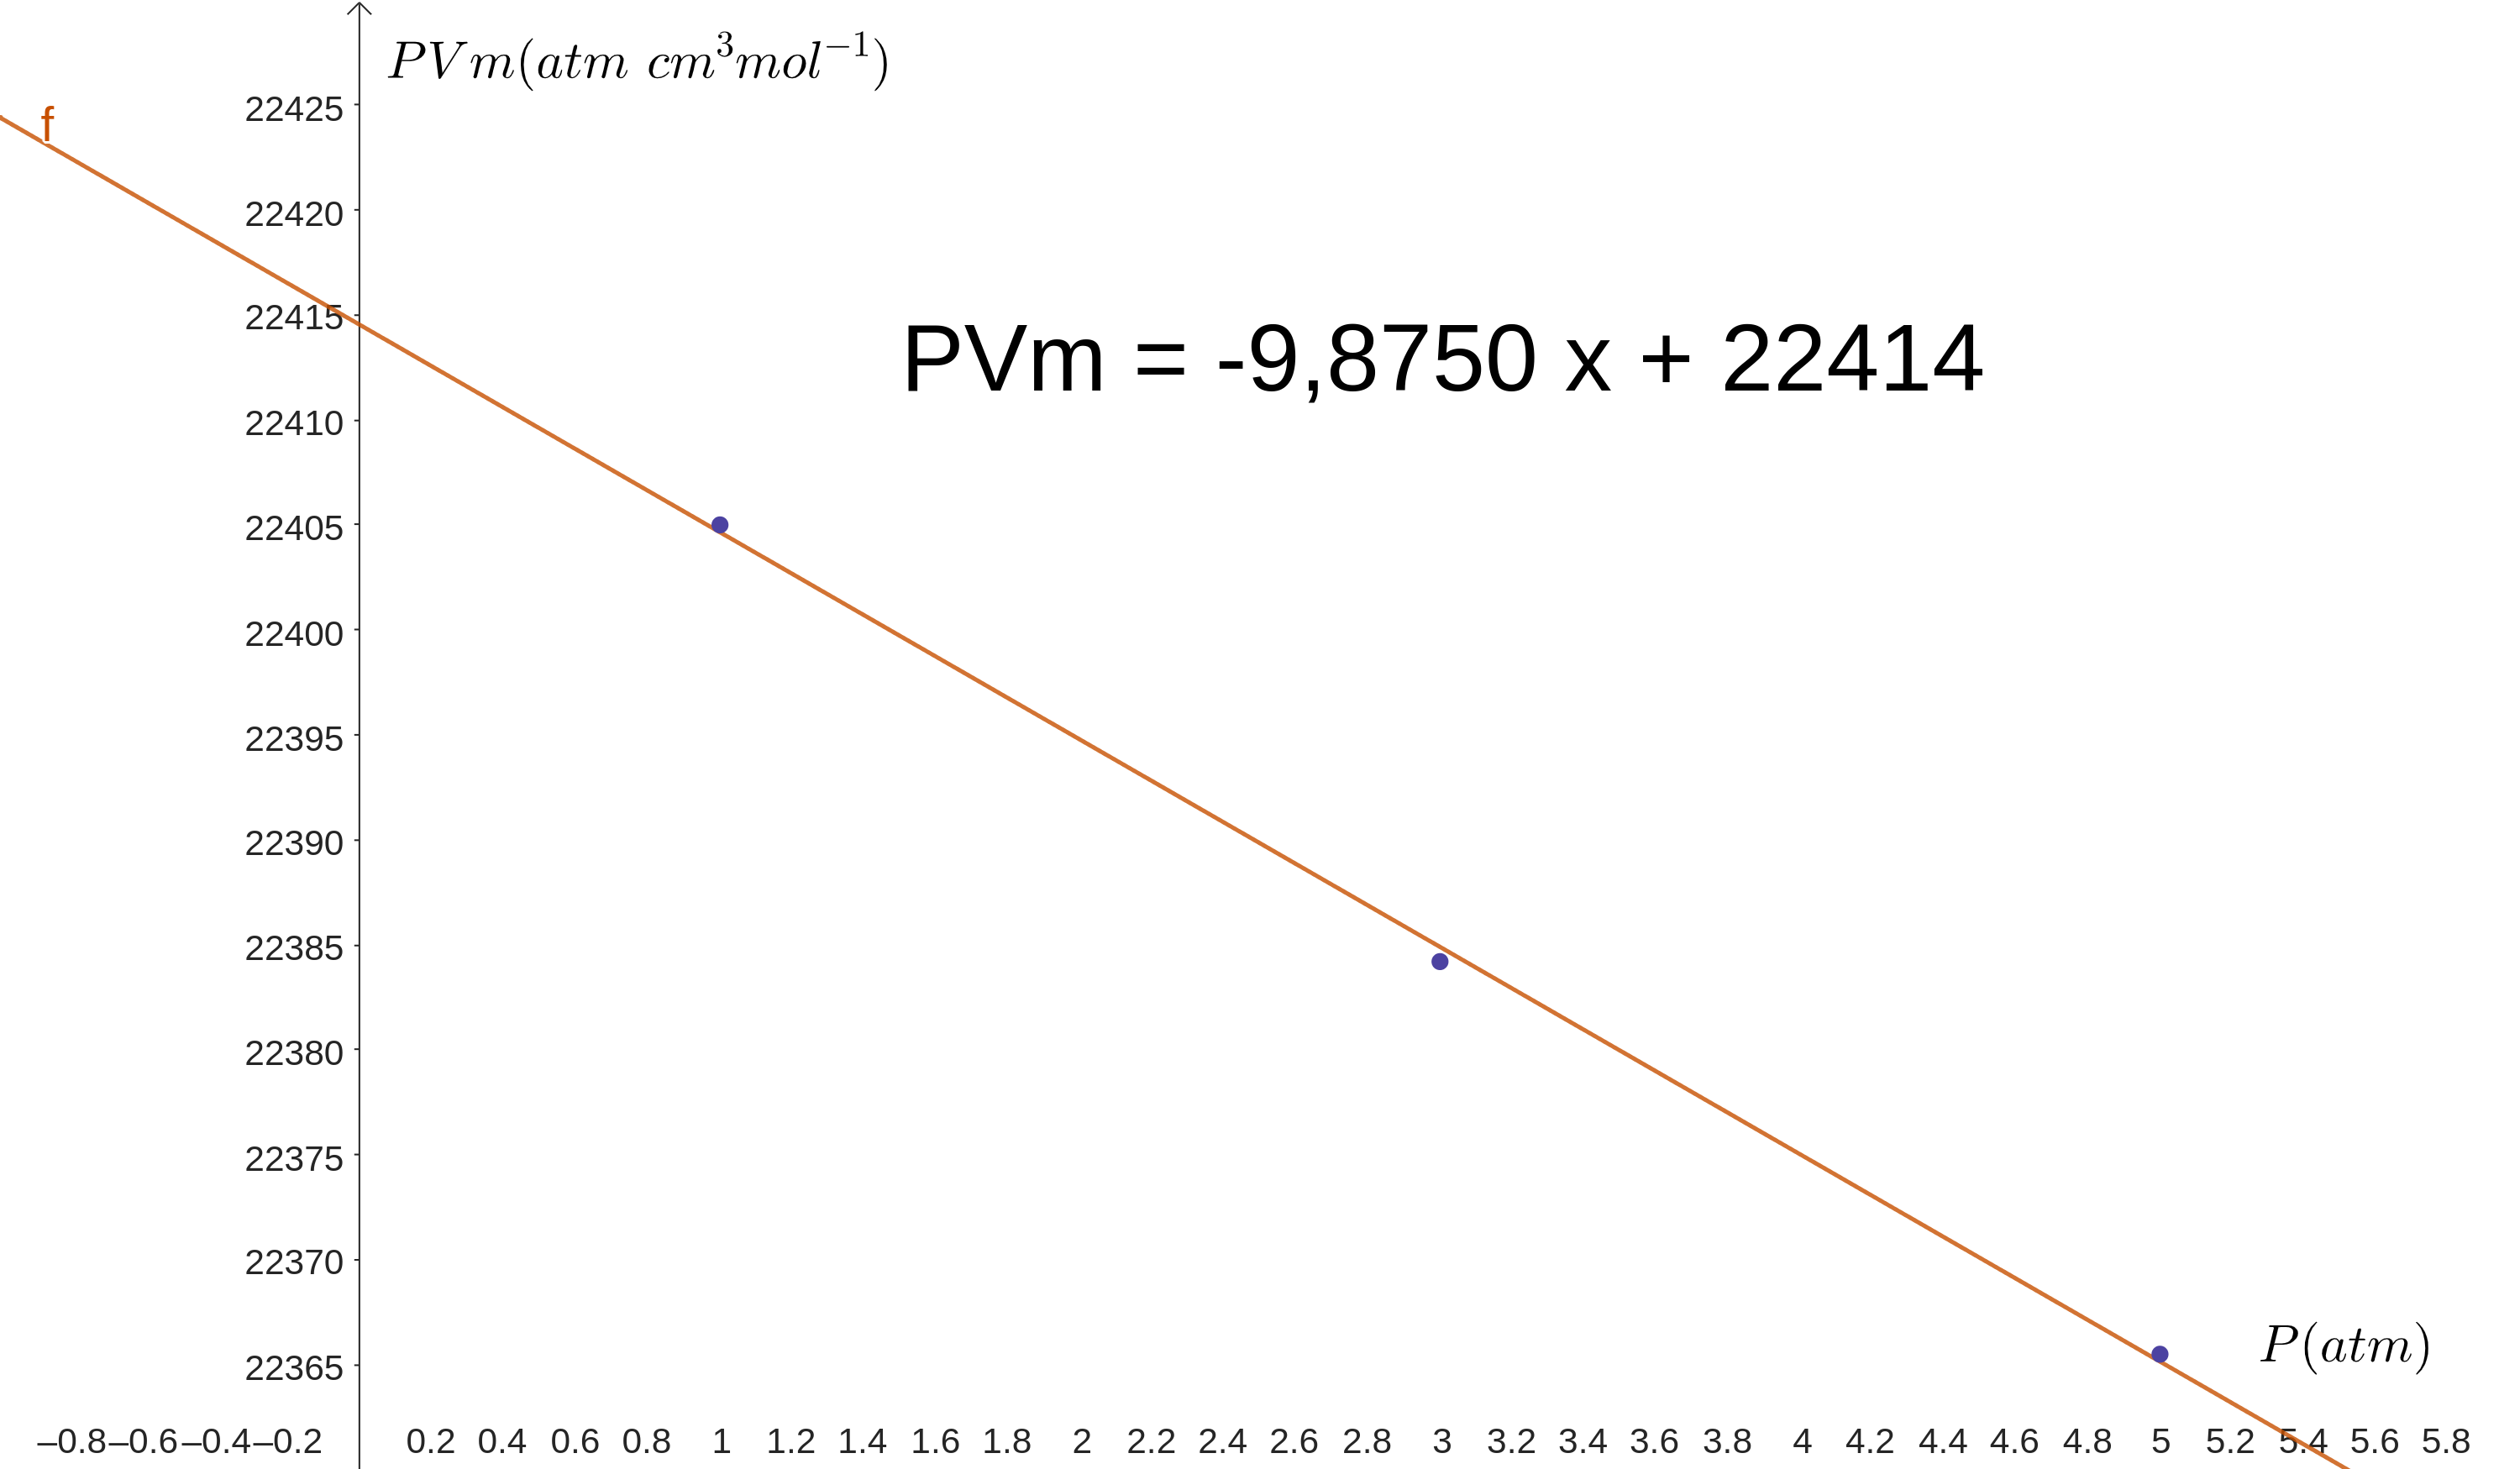
\includegraphics[width=.5\linewidth]{images/geogebra.png}
        \caption{Regressão Linear de P x \(PV_m\)}
        \label{reggeo}
    \end{figure}

    Segundo a regressão linear realizada pela ferramenta do GeoGebra, quando \(
    P \to 0 \) a função \( PV_m \) tende a \( 22414 \) atm cm\(^3\)
    mol\(^{-1}\). 
    E como mostrado anteriormente \( PV_m = RT \Rightarrow
    \frac{PV_m}{T} = R \), então:
    \begin{align*}
        22414 \, \text{atm cm}^3 \text{mol}^{-1} = R \times 273,15 \, \text{K}\\
        \Rightarrow R = \frac{22414}{273,15} \, \text{atm cm}^3
        \text{mol}^{-1} \text{K}^{-1}\\
        R = 82,057 \, \text{atm cm}^3 \text{mol}^{-1} \text{K}^{-1}
    \end{align*}
    Note que esse valor está alinhado com o valor de referência.
    
\end{rsl}
